% !TEX root = ../../../main.tex

\toggletrue{image}
\toggletrue{imagehover}
\chapterimage{data_pipeline_2x}
\chapterimagetitle{\uppercase{Data Pipeline}}
\chapterimageurl{https://xkcd.com/2054/}
\chapterimagehover{\say{Is the pipeline literally running from your laptop?} \say{Don't be silly, my laptop disconnects far too often to host a service we rely on. It's running on my phone.}}

\chapter{Benutzereingabe}
\label{ch:benutzereingabe}

Wenn wir die Rolle vom Programmierer zum \textbf{Benutzer} eines Programms wechseln, müssen wir die Möglichkeit haben, die Verarbeitung eines Programms zu beeinflussen. Ein Benutzer ist kein Programmierer und soll den Code \textbf{nicht} ändern müssen. Dies wird in der Programmierung durch eine Benutzereingabe realisiert. Bei der Turtle-Programmierung können wir uns darunter die Auswahl einer Farbe durch den Benutzer vorstellen. Die Lernziele lauten:\\

\lernziel{\autoref{ch:benutzereingabe}, \nameref{ch:benutzereingabe}}{
\begin{minipage}{\linewidth}
$\square$ \hspace{0.1cm} Sie erstellen ein Programm, das dem Benutzer die Eingabe eines Floats ermöglicht.\\
$\square$ \hspace{0.1cm} Sie erstellen ein Programm, das dem Benutzer die Eingabe eines Strings ermöglicht.\\
$\square$ \hspace{0.1cm} Sie erstellen ein Programm, das dem Benutzer die Eingabe eines Integers ermöglicht.
\end{minipage}
}

\section{Die Benutzereingabe von Floats}

Mit der Funktion \lstinline[language={python3}]{numinput} des Turtle-Moduls\footnote{\lstinline[language={python3}]{numinput} ist vermutlich eine Abkürzung für \textit{numerical input}.} kann der Benutzer zur Eingabe einer \textbf{Zahl} aufgefordert werden. \autoref{lst:numinput-1} zeigt ein Beispiel. In Zeile drei wird der Funktionsaufruf durchgeführt.

\begin{lstlisting}[language={python3}, label={lst:numinput-1}, caption={Wenn wir das Programm ausführen, dann öffnet sich ein Fenster für die Eingabe.}]
import turtle as t

a = t.numinput("Quadrat", "Bitte geben Sie die Seitenlänge ein:")
for _ in range(4):
	t.forward(a)
	t.left(90)
t.done()

\end{lstlisting}

Mit der Funktion \lstinline[language={python3}]{numinput} kann der Benutzer eine \textbf{beliebige Zahl} eingeben.

\begin{important}
	Wenn wir ein Programm mit einem \lstinline[language={python3}]{numinput}-Funktionsaufruf ausführen, dann wird das Programm in der Zeile mit dem \lstinline[language={python3}]{numinput}-Funktionsaufruf \textbf{automatisch angehalten}. Es geht erst dann \textbf{weiter}, wenn der Benutzer die Eingabe mit \textbf{\say{OK}} bestätigt.
\end{important}

Die Benutzereingabe können wir dann in einer Variablen speichern. In \autoref{lst:numinput-1} wird die Eingabe in der Variablen \lstinline[language={python3}]{a} gespeichert. Wenn wir \lstinline[language={python3}]{numinput} verwenden, dann wird \textbf{immer ein Float} erzeugt. Auch dann, wenn wir \say{eine Zahl ohne Punkt} eingeben.

\subsection{Argumente der  \lstinline[language={python3}]{numinput}-Funktion}
\label{subsec:numinput-argumente}

Die \lstinline[language={python3}]{numinput}-Funktion wird typischerweise mit zwei Argumenten aufgerufen:

\begin{itemize}
\item Das \textbf{erste Argument} bestimmt den \textbf{Titel} des Fensters.
\item Das \textbf{zweite Argument} bestimmt den \textbf{Inhalt} des Fensters.
\end{itemize}

Beide Argumente müssen ein \textbf{String} sein.

\begin{example}
In \autoref{figure:numinput-1} ist das Fenster zum Code aus \autoref{lst:numinput-1} (Zeile 3) gezeigt.
\end{example}

\begin{figure}[H]
\centering
\begin{minipage}{0.45\textwidth}
\centering
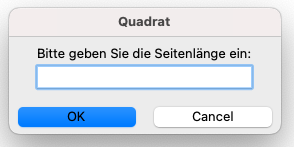
\includegraphics[width=\textwidth]{input_quadrat}
\caption{Fenster für die Benutzereingabe. Der Screenshot wurde unter macOS gemacht.\protect\footnotemark}
\label{figure:numinput-1}
\end{minipage}
\hfill
\begin{minipage}{0.45\textwidth}
\centering
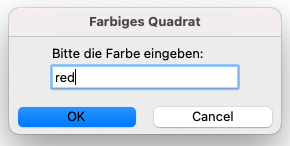
\includegraphics[width=\textwidth]{input_farbiges_quadrat}
\caption{Bei einer Texteingabe dürfen die doppelten Anführungszeichen nicht eingegeben werden.\protect\footnotemark}
\label{figure:textinput-1}
\end{minipage}
\end{figure}

\footnotetext{Bildquelle: Screenshot des Programms.}
\footnotetext{Bildquelle: Screenshot des Programms.}

\section{Die Benutzereingabe von Strings}

Mit der Funktion \lstinline[language={python3}]{textinput} des Turtle-Moduls kann der Benutzer zur Texteingabe aufgefordert werden. \autoref{lst:textinput-1} zeigt ein Beispiel. In Zeile drei wird der Funktionsaufruf durchgeführt.

\begin{lstlisting}[language={python3}, label={lst:textinput-1}, caption={Das Konzept für die Benutzereingabe eines Strings ist praktisch identisch mit dem Konzept für die Benutzereingabe eines Floats.}]
import turtle as t

farbe = t.textinput("Farbiges Quadrat", "Bitte die Farbe eingeben:")
t.pencolor(farbe)
for _ in range(4):
	t.forward(200)
	t.left(90)
t.done()

\end{lstlisting}

Auch bei \lstinline[language={python3}]{textinput} wird das Programm angehalten und der Benutzer muss mit \say{OK} die Eingabe bestätigen. Die Argumente der \lstinline[language={python3}]{textinput} sind identisch zur \lstinline[language={python3}]{numinput}-Funktion.

\begin{important}
Wenn wir mit \lstinline{textinput} etwas eintippen, dann benötigen wir für die Eingabe \textbf{keine doppelten Anführungszeichen}.
\end{important}

In \autoref{lst:textinput-1} speichert die Variable \lstinline[language={python3}]{farbe} somit nach der Eingabe einen \textbf{String}.

\begin{example}
In \autoref{figure:textinput-1} ist das Fenster zum Code aus \autoref{lst:textinput-1} (Zeile 3) gezeigt. Die Texteingabe erfolgt \textbf{ohne} doppelte Anführungszeichen.
\end{example}

Wir können natürlich auch eine Texteingabe mit der Benutzereingabe für eine Zahl kombinieren. Es ist auch möglich, mehrere Benutzereingaben einzubauen oder eine wiederholte Benutzereingabe in einer Schleife zu verwenden.

\section{Die Benutzereingabe von Integers}

Wollen wir den Benutzer nach einer ganzen Zahl fragen, dann benötigen wir die \lstinline[language={python3}]{numinput}-Funktion in Kombination mit der \lstinline[language={python3}]{int}-Funktion.

\begin{lstlisting}[language={python3}, label={lst:numinput-2}, caption={Wir können eine Variable als Zwischenspeicher für die Eingabe verwenden oder die Funktionsaufrufe verschachteln (Auszug aus dem Quellcode).}]
import turtle as t
import random as r

# Erste Möglichkeit
eingabe = t.numinput("Zufallsquadrat", "Minimale Seitenlänge:")
min_laenge = int(eingabe)

# Zweite Möglichkeit
max_laenge = int(t.numinput("Zufallsquadrat", "Maximale Seitenlänge:"))

seitenlaenge = r.randrange(min_laenge, max_laenge + 1)
\end{lstlisting}

Die \lstinline[language={python3}]{int}-Funktion konstruiert aus einem Float einen Integer. Bei der Konstruktion werden alle Nachkommastellen ignoriert und nur die \textbf{Zahl vor dem Komma} wird zur Erzeugung des Integers verwendet. Es wird \textbf{nicht} gerundet.

\begin{important}
Auch wenn Sie in der Benutzereingabe einen Float mit einem Punkt eingeben, die \lstinline[language={python3}]{int}-Funktion konstruiert daraus einen Integer und schneidet alle Nachkommastellen \say{ab}.
\end{important}

\subsection{Verschachtelte Funktionsaufrufe}

Wir können zwei Funktionsaufrufe verschachteln, wenn der \textbf{erste Funktionsaufruf} einen Wert erzeugt. Wir sagen, die \textbf{Funktion gibt einen Wert zurück}. Wir können dann den \textbf{Funktionsaufruf als Argument} für den \textbf{zweiten Funktionsaufruf} verwenden.

\begin{example}
\autoref{lst:nested-function-calls} zeigt ein paar verschachtelte Funktionsaufrufe.

\begin{lstlisting}[language={python3}, label={lst:nested-function-calls}, caption={Der innere Funktionsaufruf erzeugt jeweils einen Wert.}]
import turtle as t
import random as r

t.pencolor(r.choice(["red", "green", "blue"]))
t.pensize(r.randrange(1, 11))
seitenlaenge = int(t.numinput("Eingabe", "Seitenlänge:"))

\end{lstlisting}

\end{example}

\vspace{-0.5cm}

\cleancoderegel{\autoref{ch:benutzereingabe}, \nameref{ch:benutzereingabe}}{
\begin{cleancode}[Verschachtelte Funktionsaufrufe]
Verschachtelte Funktionsaufrufe mit Vorsicht verwenden! Das Programm \textbf{muss korrekt und lesbar} bleiben.
\end{cleancode}
}

\vspace{-0.5cm}

\subsection{Eingebaute Funktionen}

Damit wir die \lstinline[language={python3}]{int}-Funktion verwenden können, benötigen wir \textbf{keine} \lstinline[language={python3}]{import}-Anweisung. Die \lstinline[language={python3}]{int}-Funktion steht jederzeit und überall zur Verfügung. Es ist eine so genannte \textbf{eingebaute Funktion} (engl. built-in function). Python stellt diese Funktionen automatisch zur Verfügung. Es gibt ungefähr \num{70} eingebaute Funktionen.

\begin{hinweis}
Im Kapitel über Schleifen haben wir bereits eine eingebaute Funktion gesehen -- die \lstinline[language={python3}]{range}-Funktion. Auch diese Funktion können wir ohne \lstinline[language={python3}]{import}-Anweisung verwenden.
\end{hinweis}

